%Organizacion UML, BPMN, OCL, BPEL4ws (archivos html estan....)
% <<notaciones y estandares utilizados>>


%--------------------------------------------------
En \'este capitulo se describir\'a la forma en la que el sistema se encuentra estructurado mediante diagramas de clase, BPMN y diagramas de secuencia.
%---------------------------------------------------------
\section{Diagrama de clases}
%---------------------------------------------------------
\section{BPMN}
El siguiente diagrama BMPN muestra el funcionamiento de la clinica con nuestro sistema ya implementado, creando mejoras significativas para la clinica.
\begin{figure}[htbp!]
\centering
		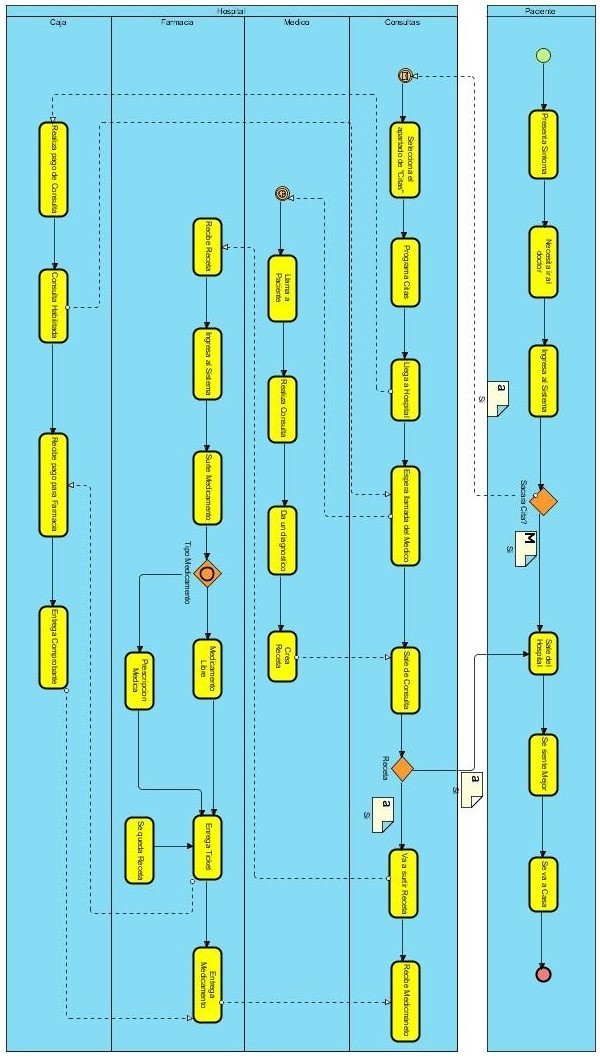
\includegraphics[width=.7\textwidth]{images/diagramabpm}
		\caption{Figura 1.1 Diagrama BPMN (Despues de Implemntar el Sistema)}
	\end{figure}
	\newpage

%---------------------------------------------------------
\section{Diagramas de secuencia}
\cfinput{diagramas/Login}
\cfinput{diagramas/Compra}
\cfinput{diagramas/Busqueda}
\cfinput{diagramas/CreaExp}
\cfinput{diagramas/ModificaExp}
\cfinput{diagramas/Receta}
\cfinput{diagramas/AgregarMed}
\cfinput{diagramas/RegMed}
\cfinput{diagramas/RegUsuario}
%---------------------------------------------------------